\documentclass[10pt,a4paper]{article}

% -------------------- PACKAGES --------------------
\usepackage[utf8]{inputenc}
\usepackage[T1]{fontenc}
\usepackage{amsmath}
\usepackage{geometry}
\geometry{margin=1in, columnsep=0.6cm}
\usepackage{graphicx}
\usepackage{xcolor}
\usepackage{listings}
\usepackage{hyperref}
\usepackage{booktabs}
\usepackage{caption}
\usepackage{float}
\usepackage{tikz}
\usetikzlibrary{arrows.meta, positioning}

% -------------------- CODE STYLING --------------------
\definecolor{codebg}{rgb}{0.95,0.95,0.97}
\lstdefinestyle{python}{
    language=Python,
    backgroundcolor=\color{codebg},
    basicstyle=\ttfamily\footnotesize,
    keywordstyle=\color{blue}\bfseries,
    commentstyle=\color{green!40!black},
    stringstyle=\color{red!60!black},
    numberstyle=\tiny\color{gray},
    breaklines=true,
    frame=single,
    tabsize=4,
    showstringspaces=false,
    xleftmargin=0.1cm,
    xrightmargin=0.1cm
}

% -------------------- DOCUMENT --------------------
\begin{document}

\title{\textbf{Autonomous Digital Terrarium: An AI-Director Multi-Agent Ecosystem with Hosted Open-Weight Models on a Minimal Container}}
\author{\href{https://github.com/Yato0226}{github.com/Yato0226}}
\maketitle

\begin{abstract}
Running persistent LLM applications on a small home server requires keeping host RAM and compute footprints minimal without sacrificing model capability. This paper demonstrates the implementation of an autonomous multi-agent ecosystem (``Digital Terrarium'') running continuously in a low-resource environment. All language-model work is offloaded to Google's hosted Gemini API, which serves the open-weight Gemma 4 family, a 31B dense model (\texttt{gemma-4-31b-it}) as the primary narrator with automatic fallback to the 26B MoE variant (\texttt{gemma-4-26b-a4b-it}), so the host needs only a 2 GB LXC container on a Proxmox VE hypervisor and no local inference hardware. The system adopts an \emph{AI Director} pattern: the LLM proposes behavioural intent for each agent, while a deterministic Python engine owns all state consequences. Per-tick, \texttt{schema.py} rebuilds a Pydantic model from the current active-agent roster, embedding one \texttt{AgentDecision} field per pawn with \texttt{action}, \texttt{narrative}, \texttt{quote}, \texttt{inner\_monologue}, \texttt{direction} (for Move), \texttt{target} (for Attack/Share/Mate, built from \texttt{Literal[tuple(pawn\_ids)]} per PEP 586 Python 3.10 compatibility), a free-form \texttt{flavor} verb (for the open-ended \texttt{Interact} action), and a \texttt{new\_goal} wish the engine may adopt into a tracked personal goal. This schema is passed to the Gemini API as a structured-output schema (\texttt{response\_schema}), which both forces valid JSON and suppresses the model's reasoning channel. The response is validated again with Pydantic, and any failed parse skips mutation and increments the tick. Any \texttt{!order} placed by the god replaces the LLM's proposed action for that agent, Python enforces it, and the LLM merely narrates. The world is exposed through a Discord bot that lets a ``god'' spawn agents, edit stats, and issue enforced orders. With the model no longer resident on the host, memory is flat and Out-Of-Memory (OOM) faults are structurally impossible; daily quota headroom, structured-output reliability, and coherent agent interactions are evaluated over extended runs.
\end{abstract}

\section{Introduction}
Running persistent LLM applications in edge environments requires strictly balancing parameter size, context management, and host system RAM allocation. Unconstrained context windows or pure text generation often result in state hallucination, numerical drift, and memory exhaustion.

This paper outlines the architecture and deployment of an autonomous ``Digital Terrarium'', a multi-agent ecosystem driven by periodic tick-based LLM calls. A key design decision is the separation of \emph{intent} from \emph{consequence}: the LLM decides what each agent \emph{wants} to do, and a deterministic engine (pure Python) validates, costs, and applies the resulting effects. Because the model never emits stat deltas, the LLM cannot corrupt the simulation; it operates strictly as the narrator and decision-maker. A novel contribution is the combination of (i) a per-tick rebuilt output schema derived from the live agent roster, and (ii) a ring buffer of structured events that lets agents react to recent history without exploding the context window. A Discord-based ``god'' interface further allows a human operator to intervene: spawning agents, editing attributes, and issuing enforced orders that override model behaviour.

\section{System Setup}

\subsection{Hardware \& Environment Specifications}
The production environment operates within a Linux Container (LXC) hosted on a Proxmox Virtual Environment (PVE) node. System resources are detailed in Table~\ref{tab:hardware}.

\begin{table}[htbp]
\centering
\caption{Host and Container Resource Allocations}
\label{tab:hardware}
\begin{tabular}{@{}ll@{}}
\toprule
\textbf{Component} & \textbf{Specification / Allocation} \\
\midrule
Host CPU & AMD Ryzen 5 5600G (6C/12T) \\
Host RAM & 16 GB DDR4 \\
Target Storage & Mechanical Hard Disk Drive (HDD) \\
LXC OS & Debian 12 / Ubuntu 22.04 LTS \\
Container RAM & 2048 MB (Allocated) \\
Container Swap & 512 MB \\
LLM Engine & Google Gemini API (hosted, off-host inference) \\
Base Model & Gemma 4 31B (\texttt{gemma-4-31b-it}), fallback Gemma 4 26B MoE (\texttt{gemma-4-26b-a4b-it}) \\
Discord API & discord.py (2.x, Message Content Intent) \\
\bottomrule
\end{tabular}
\end{table}

\subsection{Architecture \& Data Pipeline}
Figure~\ref{fig:architecture} shows the overall system: the AI Director sits between the world it observes and the engine that resolves its intentions, with the ``god'' above all three. Every tick flows through the pipeline in Figure~\ref{fig:tick}.

\begin{figure}[htbp]
\centering
\resizebox{\textwidth}{!}{%
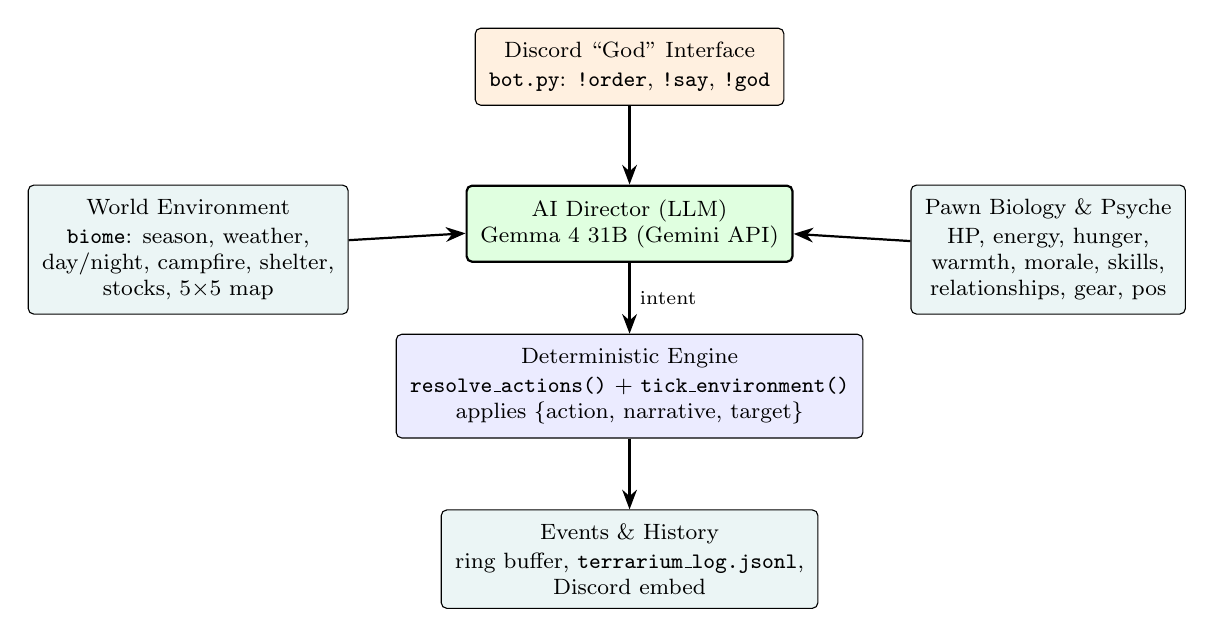
\begin{tikzpicture}[
    node distance=0.9cm,
    box/.style={draw, rounded corners=2pt, align=center, inner sep=5pt, font=\footnotesize},
    llm/.style={box, fill=green!12, thick},
    god/.style={box, fill=orange!12},
    world/.style={box, fill=teal!8},
    engine/.style={box, fill=blue!8},
    arrow/.style={-{Stealth[length=2.5mm]}, thick},
]
    \node[god] (god) {Discord ``God'' Interface\\[1pt] \texttt{bot.py}: \texttt{!order}, \texttt{!say}, \texttt{!god}};
    \node[world, below left=1.0cm and 1.6cm of god] (env) {World Environment\\[1pt] \texttt{biome}: season, weather,\\ day/night, campfire, shelter,\\ stocks, 5$\times$5 map};
    \node[world, below right=1.0cm and 1.6cm of god] (pawn) {Pawn Biology \& Psyche\\[1pt] HP, energy, hunger,\\ warmth, morale, skills,\\ relationships, gear, pos};
    \node[llm, below=1.0cm of god] (llm) {AI Director (LLM)\\ Gemma 4 31B (Gemini API)};
    \node[engine, below=0.9cm of llm] (engine) {Deterministic Engine\\[1pt] \texttt{resolve\_actions()} + \texttt{tick\_environment()}\\ applies \{action, narrative, target\}};
    \node[world, below=0.9cm of engine] (events) {Events \& History\\[1pt] ring buffer, \texttt{terrarium\_log.jsonl},\\ Discord embed};

    \draw[arrow] (god) -- (llm);
    \draw[arrow] (env) -- (llm);
    \draw[arrow] (pawn) -- (llm);
    \draw[arrow] (llm) -- node[right, font=\scriptsize] {intent} (engine);
    \draw[arrow] (engine) -- (events);
\end{tikzpicture}}%
\caption{AI Director system architecture. The LLM proposes intent; a deterministic Python engine owns all consequences. Per-tick schema rebuild in \texttt{schema.py} is roster-aware via \texttt{Literal[tuple(pawn\_ids)]} (Python 3.10 compatibility). Slow I/O (eulogy LLM, Discord embed) runs outside the tick lock.}
\label{fig:architecture}
\end{figure}

The system is a single Python process split into focused modules: \texttt{state.py} (world state and persistence), \texttt{schema.py} (per-tick LLM output models), \texttt{prompts.py} (system prompt and prompt builder), \texttt{llm.py} (hosted Gemini API client with primary/fallback models), \texttt{engine.py} (deterministic rules), \texttt{events.py} (structured event log), \texttt{core.py} (tick orchestration and scheduler), and \texttt{bot.py} (Discord god interface). The data flow per tick is:

\begin{enumerate}
\item \textbf{Schema rebuild}: \texttt{schema.py} constructs a Pydantic model containing one decision field per \emph{active} agent, plus optional \texttt{quote}, \texttt{inner\_monologue}, and Move \texttt{direction} fields and a \texttt{target} literal built from the current roster. Adding or removing agents therefore requires no schema edits.
\item \textbf{Decision}: the LLM is prompted with current vitals, skills, personality, relationships, gear, map positions, and the event ring buffer. The per-tick Pydantic schema is passed to the API as a structured-output schema (\texttt{response\_schema}) that both forces valid JSON and suppresses the model's reasoning channel; the response is validated again with Pydantic, and a failed parse skips mutation and increments the tick.
\item \textbf{Intent override}: any \texttt{!order} placed by the god replaces the LLM's proposed action for that agent, Python enforces it, the LLM merely narrates.
\item \textbf{Deterministic resolution}: \texttt{engine.resolve\_actions()} validates the intent (energy cost, target legality), computes consequences (damage, resources, skill XP, relationship deltas), and emits structured events.
\item \textbf{Save inside lock}: \texttt{terrarium\_state.json} is persisted (auto-migrated on startup), the tick counter is incremented, and the tick lock is released. Then the best-effort eulogy LLM generates tombstone inscriptions for the newly fallen, and a formatted Discord embed is posted outside the lock so god commands are not stalled by network I/O.
\end{enumerate}

\begin{figure}[htbp]
\centering
\resizebox{\textwidth}{!}{%
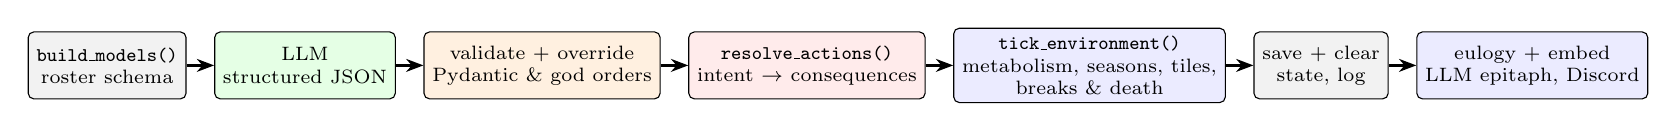
\begin{tikzpicture}[
    node distance=0.55cm and 0.35cm,
    stage/.style={draw, rounded corners=2pt, align=center,
                  minimum height=0.85cm, inner sep=3pt, font=\scriptsize},
    arrow/.style={-{Stealth[length=2.2mm]}, thick},
]
    \node[stage, fill=gray!10] (s1) {\texttt{build\_models()}\\roster schema};
    \node[stage, right=of s1, fill=green!10] (s2) {LLM\\structured JSON};
    \node[stage, right=of s2, fill=orange!12] (s3) {validate + override\\Pydantic \& god orders};
    \node[stage, right=of s3, fill=red!8] (s4) {\texttt{resolve\_actions()}\\intent $\to$ consequences};
    \node[stage, right=of s4, fill=blue!8] (s5) {\texttt{tick\_environment()}\\metabolism, seasons, tiles,\\ breaks \& death};
    \node[stage, right=of s5, fill=gray!10] (s6) {save + clear\\state, log};
    \node[stage, right=of s6, fill=blue!8] (s7) {eulogy + embed\\LLM epitaph, Discord};

    \foreach \a/\b in {s1/s2, s2/s3, s3/s4, s4/s5, s5/s6, s6/s7}
        \draw[arrow] (\a) -- (\b);
\end{tikzpicture}}%
\caption{Per-tick pipeline. Only the LLM step is non-deterministic; everything else is deterministic Python. Save (state + log + tick increment) runs inside the lock; eulogy LLM + Discord embed run outside the lock. Pawn roster reflected in schema rebuild.}
\label{fig:tick}
\end{figure}

Agent state is intentionally rich and nested: \texttt{vitals} (HP, energy, hunger, warmth, morale), \texttt{skills} (woodcutting, scouting, combat), \texttt{personality}, \texttt{inventory} (wood, food, stone, fiber), \texttt{gear} (main hand / body equipment), \texttt{counters} (lifetime deeds such as trees felled and blizzards survived), a \texttt{title} epithet recomputed from those counters each tick, \texttt{relationships}, a \texttt{pos} coordinate on a shared $5\times5$ map, and \texttt{status} (active / incapacitated / dead). A shared \texttt{biome} block holds the world: season (rolled every 100 ticks, Figure~\ref{fig:seasons}), weather, a 20-tick day/night cycle, campfire and shelter integrity, depletable wood/food stocks that regrow every tick except in Winter, and the map tiles themselves. A lit campfire warms only agents within one tile of the Camp tile; shelter warmth is global. Reaching 0 HP incapacitates an agent; it is excluded from LLM decisions and auto-recovers 10 HP per subsequent tick. Environmental permadeath is reserved for freezing in a Blizzard (warmth reaches 0), starvation beyond five consecutive starving ticks, or reaching old age (\texttt{OLD\_AGE\_MAX} = 320 ticks = 16 days): the agent is removed from the roster and enshrined in the \texttt{graveyard} with its final epithet, cause, and a tombstone. Psychological pressure is a real mechanic: morale below 20 is a breakdown risk, morale at 0 triggers a deterministic \emph{mental break} (berserk rampage, paranoid hiding, or apathetic wandering) that overrides all agency for three ticks, and morale above 80 grants a $+10\%$ gathering bonus. All action effects are listed in Table~\ref{tab:actions}; the LLM's schema contains \emph{no} numerical fields.

\begin{figure}[htbp]
\centering
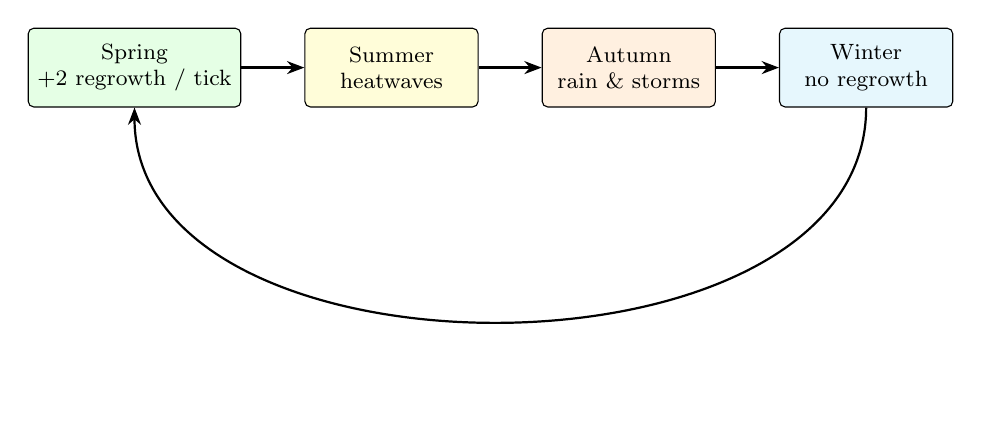
\begin{tikzpicture}[
    node distance=0.8cm,
    season/.style={draw, rounded corners=2pt, align=center,
                   minimum height=1.0cm, minimum width=2.2cm,
                   font=\footnotesize},
    arrow/.style={-{Stealth[length=2.2mm]}, thick},
]
    \node[season, fill=green!10] (spring) {Spring\\+2 regrowth / tick};
    \node[season, right=of spring, fill=yellow!15] (summer) {Summer\\heatwaves};
    \node[season, right=of summer, fill=orange!12] (autumn) {Autumn\\rain \& storms};
    \node[season, right=of autumn, fill=cyan!10] (winter) {Winter\\no regrowth};
    \draw[arrow] (spring) -- (summer);
    \draw[arrow] (summer) -- (autumn);
    \draw[arrow] (autumn) -- (winter);
    \draw[arrow] (winter.south) to[out=270, in=270] (spring.south);
\end{tikzpicture}
\caption{Seasonal cycle: one season every 100 ticks. Winter halts regrowth and makes warmth critical.}
\label{fig:seasons}
\end{figure}

\begin{table}[htbp]
\centering
\caption{Deterministic Action Rules (engine.py)}
\label{tab:actions}
\small
\begin{tabular}{@{}llp{0.55\textwidth}@{}}
\toprule
\textbf{Action} & \textbf{Energy Cost} & \textbf{Engine Effect} \\
\midrule
Rest   & 0  & +10 HP, +20 energy \\
Chop   & 10 & Forest tiles only; +3--7 wood (scaled by woodcutting), depletes \texttt{wood\_stock}, +1 woodcutting XP; Stone Axe doubles the yield \\
Scout  & 15 & chance of +2--6 food (scaled by scouting), +1 scouting XP; Ruins give richer loot with a stumble risk; Quarry yields stone \\
Forage & 10 & Meadow/River tiles only; +2--6 food (capped by \texttt{food\_stock}), depletes stock, +1 scouting XP; Meadows also yield fiber \\
Build  & 15 & Camp tile only; auto-crafts the best affordable tool (Stone Axe 3W+2S, Flint Spear 2W+1S, Warm Coat 5F) before spending 3 wood on +8 shelter/campfire \\
Share  & 5  & same/adjacent tile; transfer 1 food to target; +25 relationship and +5 morale for both \\
Attack & 20 & same/adjacent tile; damage $= \max(1,\ 5 + \lfloor \text{combat}/2 \rfloor - \lfloor \text{target.combat}/4 \rfloor)$; Flint Spear adds 4; $-10/-15$ relationship deltas, +1 combat XP \\
Move   & 5  & travel one tile N/S/E/W within the $5\times5$ grid; positions gate Chop/Forage/Build and close the distance for Attack/Share \\
Interact & 5 & any free-form verb in \texttt{flavor}; engine buckets it by keyword: social (+5 morale, $\pm$10 relationship with a same-tile pawn), gather (small tile-gated yield), craft (+3 shelter at Camp), relax (+10 energy, +3 morale), train (+1 combat XP); unknown verbs still grant a safe +3 morale \\
\bottomrule
\end{tabular}
\caption*{\scriptsize All yields receive a $+10\%$ bonus while morale is above 80 (``Inspired''). Personal goals (\texttt{goal}) are proposed by the LLM in \texttt{new\_goal}, parsed and tracked by the engine, advanced by matching deeds, and pay $+15$ morale and skill XP on completion.}
\end{table}

\subsection{Discord ``God'' Interface}
Beyond the one-way webhook embeds, a two-way Discord bot (prefix \texttt{!}) exposes a god layer that manipulates the world directly (Table~\ref{tab:god}). Commands that mutate \texttt{world\_state} are serialised against the tick loop via an \texttt{asyncio.Lock}, and a \texttt{!pause}/\texttt{!resume} pair gates the scheduler. Enforced orders (\texttt{!order}) are injected into the prompt and overridden in code; whispers (\texttt{!say}) are injected into the prompt \emph{and} grant a deterministic $+15$ morale, letting the Creator pull an agent out of a mental break. \texttt{!graveyard} reads the permanent record of the fallen.

\begin{table}[htbp]
\centering
\caption{God Commands (bot.py)}
\label{tab:god}
\begin{tabular}{@{}ll@{}}
\toprule
\textbf{Command} & \textbf{Effect} \\
\midrule
\texttt{!add \textless name\textgreater [hp] [energy]} & Spawn a new agent \\
\texttt{!remove \textless pawn\_id\textgreater}         & Remove an agent (never the last) \\
\texttt{!god \textless id\textgreater \textless stat\textgreater \textless v\textgreater}       & Set vitals/wood/food/stone/fiber, or \texttt{revive} \\
\texttt{!order \textless id\textgreater \textless action\textgreater [tgt]} & Enforce an action next tick (Move takes N/S/E/W) \\
\texttt{!say \textless id\textgreater \textless text\textgreater}           & Inject a whisper into the prompt; also +15 morale \\
\texttt{!graveyard}                 & List the fallen with epithets and epitaphs \\
\texttt{!status} / \texttt{!tick} / \texttt{!pause} / \texttt{!resume} & Inspect, force, or gate the simulation \\
\bottomrule
\end{tabular}
\end{table}

\subsection{Implementation Code}
Listing~\ref{lst:schema} shows the per-tick dynamic schema; Listing~\ref{lst:engine} the deterministic resolution core; Listing~\ref{lst:tick} the tick orchestration. Together they implement the AI Director pattern. Note that \texttt{Literal[tuple(pawn\_ids)]} is used deliberately: on Python 3.10 the starred \texttt{Literal[*ids]} unpacking form is unavailable, and the tuple form is equivalent per PEP~586.

\begin{lstlisting}[style=python, caption={Dynamic LLM Output Schema (schema.py, condensed). Uses \texttt{Literal[tuple(pawn\_ids)]} for Python 3.10 compatibility (PEP 586)}, label={lst:schema}]
def build_models():
    pawn_ids = [pid for pid, p in world_state["pawns"].items()
                if p["status"] == "active"]            # roster-aware
    AgentDecision = create_model(
        "AgentDecision",
        action=(Literal["Chop", "Rest", "Scout", "Attack", "Forage", "Build", "Share", "Move", "Mate", "Interact"],
                Field(description="Intent")),
        narrative=(str, Field(description="1-2 sentence narrative")),
        quote=(Optional[str], Field(default=None, description="Outward speech")),
        inner_monologue=(Optional[str], Field(default=None,
                                              description="Private thought")),
        direction=(Optional[Literal["N", "S", "E", "W"]], Field(
            default=None, description="Direction - only for Move")),
        target=(Optional[Literal[tuple(pawn_ids)]], Field(
            default=None, description="Target pawn id - for Attack/Share/Mate")),
        flavor=(Optional[str], Field(default=None,
                                     description="Free-form verb - only for Interact")),
        new_goal=(Optional[str], Field(default=None,
                                       description="Personal goal wish when goal-less")),
    )
    fields = {"world_event": (str, Field(description="Global status"))}
    for pid in pawn_ids:                               # one field per active pawn
        fields[pid] = (AgentDecision, Field(description=f"Decision for {pid}"))
    return create_model("TickResponse", **fields)
\end{lstlisting}

\begin{lstlisting}[style=python, caption={Deterministic Resolution (engine.py, condensed). Applies action $\to$ consequences: energy costs, combat, skill XP, relationships, incapacitation, crafting, mental breaks, environmental death, Mate, free-form Interact, and personal goals}, label={lst:engine}]
def resolve_actions(intents):
    for pawn_id, intent in intents.items(): # (action, target, flavor, new_goal)
        pawn = world_state["pawns"][pawn_id]
        action = intent[0]
        target = intent[1] if len(intent) > 1 else None
        flavor = intent[2] if len(intent) > 2 else None
        cost = ACTION_COSTS[action]   # Chop 10, Scout 15, Move 5, Interact 5
        if pawn["vitals"]["energy"] < cost:        # engine refuses intent
            add_event("failed", reason="low_energy")
            continue
        pawn["vitals"]["energy"] -= cost
        if action == "Rest":
            pawn["vitals"]["hp"] += 10
        elif action == "Chop":
            if tile_at(pawn) not in FOREST: add_event("failed"); continue
            wood = min(biome["wood_stock"], 3 + pawn["skills"]["woodcutting"] // 3)
            if pawn["gear"]["main_hand"] == "Stone Axe": wood *= 2
            biome["wood_stock"] -= wood            # forest is depletable
            pawn["inventory"]["wood"] += wood
        elif action == "Move":
            if not in_bounds(pos + DIRS[direction]):
                add_event("failed", reason="off_grid"); continue
            pawn["pos"] += DIRS[direction]         # tile-gated world
        elif action == "Forage":
            if tile_at(pawn) not in (MEADOW, RIVER): add_event("failed"); continue
            food = min(biome["food_stock"], 2 + pawn["skills"]["scouting"] // 4)
            biome["food_stock"] -= food; pawn["inventory"]["food"] += food
        elif action == "Build":
            if pawn["inventory"]["wood"] < 3:
                add_event("failed", reason="need_wood"); continue
            if craft := best_affordable_tool(pawn):  # 3W+2S, 2W+1S, 5F
                give_gear(pawn, craft); add_event("craft", item=craft); continue
            biome["shelter"] = min(100, biome["shelter"] + 8)
        elif action == "Share":
            if not legal_target(target):
                add_event("failed"); continue
            pawn["inventory"]["food"] -= 1
            world_state["pawns"][target]["inventory"]["food"] += 1
        elif action == "Attack":
            if not target or target == pawn_id or not target_pawn_active(target):
                add_event("failed", reason="illegal_target")
                continue
            dmg = max(1, 5 + pawn["skills"]["combat"] // 2
                      - target["skills"]["combat"] // 4)
            target["vitals"]["hp"] = clamp(target["vitals"]["hp"] - dmg)
            if target["vitals"]["hp"] <= 0:
                target["status"] = "incapacitated" # auto-recovers next tick
        elif action == "Mate":
            if not legal_target(target):
                add_event("failed"); continue
            if target["sex"] == pawn["sex"]: ...      # opposite-sex required
            if _are_kin(pawn, target): ...            # siblings/half-siblings/parent-child blocked
                add_event("failed", reason="too_close_kin")
            if pawn_id not in target["partners"]:     # committed couples skip the bond gate
                if pawn["relationships"].get(target, 0) < MATE_RELATIONSHIP or \
                   target["relationships"].get(pawn_id, 0) < MATE_RELATIONSHIP: ...
                    # mutual consent: both directions must be 25+ (else "isn't ready")
            if random.random() < CONCEPTION_CHANCE:
                target["pregnant_ticks"] = PREGNANCY_TICKS  # 20 ticks = 1 day
                target["partner_id"] = pawn_id   # father pinned until birth
            pawn["partners"] = dedup(pawn["partners"] + [target])   # pairing is official
            target["partners"] = dedup(target["partners"] + [pawn_id])
            # relationships fade 5 steps toward 0 each dawn (RELATIONSHIP_DECAY)
        elif action == "Interact":
            # free-form verb: engine buckets it into safe effects
            if flavor in SOCIAL_WORDS:          # +5 morale; same-tile bond ±10
                pawn["vitals"]["morale"] += 5
            elif flavor in GATHER_WORDS:        # small tile-gated yield
                if tile_at(pawn) in FORAGE_TILES: food += 1  # meadow/river
                elif tile_at(pawn) in FOREST_TILES: wood += 1
                elif tile_at(pawn) in (RUIN, QUARRY): stone += 1
            elif flavor in CRAFT_WORDS:         # at Camp: shelter +3 else +5 morale
                biome["shelter"] = min(100, biome["shelter"] + 3)
            elif flavor in RELAX_WORDS:         # +10 energy, +3 morale
                pawn["vitals"]["energy"] += 10
            elif flavor in TRAIN_WORDS:         # +1 combat XP
                pawn["skills"]["combat"] += 1
            else:
                pawn["vitals"]["morale"] += 3   # unknown verb is still safe
    else:
        pawn["vitals"]["morale"] = clamp(pawn["vitals"]["morale"] - 5)
    # mental break resolution overrides intent when morale is 0
    if pawn.get("mental_break"):
        _resolve_break(pawn, pawn_id)

    # personal goals: adopt LLM wishes, advance on deeds, pay off when done
    if not pawn.get("goal") and new_goal:
        pawn["goal"] = adopt_goal(pawn, new_goal)
        #   "gather 10 wood"  -> {kind:gather, resource:wood, needed:10}
        #   "befriend Scout"  -> {kind:social, target_id:<id>}
        #   "survive 5 days"  -> {kind:survive, needed:5 * TICKS_PER_DAY}
    for pid, p in world_state["pawns"].items():
        goal = p.get("goal")
        if goal and goal["progress"] >= goal["needed"]:
            p["vitals"]["morale"] += GOAL_MORALE     # +15 and skill XP
            add_event("goal", actor=pid, goal=goal["text"])
            p["goal"] = None                          # ready for the next wish

def tick_environment():             # the world ages after pawns act
    biome = world_state["biome"]    # season, weather, day/night, stocks
    ...                             # campfire burns 1 wood per tick;
                                    # metabolism, regrowth (never in
                                    # Winter), frostbite, starvation
    # aging: elders drain +1 energy/morale/tick, heal −5 less
    if age_of(pawn) >= ELDER_AGE:       # 200 ticks = 10 days → elder
        ...                             # +1/tick energy & morale tax
        if age_of(pawn) >= OLD_AGE_MAX:  # 320 ticks = 16 days → 2% death chance
            _kill(pawn_id, pawn, "old age")
\end{lstlisting}

\begin{lstlisting}[style=python, caption={Tick Orchestration (core.py, condensed). lock $\to$ schema $\to$ LLM $\to$ override $\to$ resolve $\to$ environment $\to$ tick++ $\to$ save; eulogy + embed outside lock}, label={lst:tick}]
async def run_tick():
    async with tick_lock:                              # serialises vs god commands
        TickResponse = schema.build_models()           # 1. roster-aware schema
        content, _ = await asyncio.to_thread(          # 2. structured LLM output
            llm.generate_with_fallback,                #    (primary -> fallback)
            SYSTEM_PROMPT, build_prompt(), TickResponse, 0.7)
        data = TickResponse.model_validate_json(content)
        events.add_event("world", description=data.world_event)
        dead_tick = state.world_state["tick"]          # capture \emph{before} mutation
        # 3. Build intents; god orders override the LLM's proposal.
        intents = {}
        for pid, pawn in state.world_state["pawns"].items():
            if pawn["status"] != "active":
                continue
            decision = getattr(data, pid)
            action, target = decision.action, decision.target
            if action == "Move":
                target = decision.direction            # map \texttt{direction}→target
            order = state.god_orders.get(pid)
            if order:
                action, target = order["action"], order.get("target")
            intents[pid] = (action, target)
        engine.resolve_actions(intents)                # 4. deterministic effects
        engine.tick_environment()                      #    world ages
        state.god_orders.clear(); state.god_whispers.clear()
        state.world_state["tick"] += 1                 # increment \emph{before} save
        state.save_state(); events.log_to_jsonl()      # 5. persist
    # Lock released: god commands can run during the slow LLM/webhook I/O.
    await _eulogize_fallen(dead_tick)                  # LLM epitaph (per fallen)
    state.save_state()                                 # re-save after eulogies
    await asyncio.to_thread(post_to_discord, data)     # Discord webhook
\end{lstlisting}

\section{Expected Outcomes}

\subsection{Design Objectives}
The AI Director architecture is evaluated against four design objectives that follow from the constraints of a 2 GB container on HDD storage:

\begin{enumerate}
\item \textbf{Zero Memory Growth}: the prompt is bounded (fixed system prompt, history truncated to the last ten structured events) and the output schema caps the response size; because inference is off-host, no KV cache or model weights occupy container RAM and memory consumption remains flat indefinitely.
\item \textbf{Deterministic Boundaries}: the model emits only \emph{intent} (action, narrative, target); all numbers are produced by the engine and clamped to \([0,100]\), so hallucinated stats are structurally impossible.
\item \textbf{Enforced Intervention}: god orders are overridden in Python after the LLM responds, so intervention is guaranteed regardless of model compliance; failed intents (energy shortfall, self-attack, missing target) are logged as \texttt{failed} events.
\item \textbf{Agent Reactivity}: each agent sees the others' vitals, skills, relationships, and recent events, enabling emergent behaviours and grudges. Relationship deltas persist across ticks but fade several steps toward zero each dawn, so bonds and feuds both require real upkeep to endure. A successful \texttt{Mate} officially pairs two pawns (recorded in each other's \texttt{partners}; polygamy allowed), and children record their parents (\texttt{mother\_id}/\texttt{father\_id}); the engine blocks incest at the mate gate. A read-only family tree (\texttt{!tree}) renders couples (mutually partnered or with shared children), mate-eligible bonds, kin lines, and rivalries from these pairwise relationships.
\end{enumerate}

\section{Results \& Evaluation}

\subsection{Performance Metrics}
When deployed inside the designated 2 GB LXC container on the Ryzen 5 5600G host, the observed execution metrics are summarised in Table~\ref{tab:metrics}. Every tick is a single \texttt{generateContent} request to the hosted Gemini API carrying a structured-output schema; the only host-side costs are the Python process, the Discord client, and the request/response. Free-tier quotas (30 RPM / 16K TPM / 14.4K RPD, resetting at midnight Pacific) bound sustained operation; at the default 60-second tick interval the daily request quota is used at roughly 10\%, leaving ample headroom for eulogies and god commands, and closing the server stops all usage.

\begin{table}[htbp]
\centering
\caption{Observed Operational Performance}
\label{tab:metrics}
\begin{tabular}{@{}ll@{}}
\toprule
\textbf{Metric} & \textbf{Observed Value} \\
\midrule
Model RAM Footprint & n/a (off-host, served by Gemini API) \\
Total Container Memory & $\approx$ 250 MB (incl. OS + bot + SDK) \\
Container Headroom & $\approx$ 1.8 GB \\
Inference Speed & hosted (off-host); 31B dense / 26B MoE via API \\
Avg. Tick Evaluation Latency & API round-trip + $<$ 0.1 s deterministic engine \\
Structured-Output Parse Failure & 0.0\% (schema-enforced, Pydantic re-validated) \\
Daily Quota Utilisation (RPD) & $\approx$ 10\% of 14.4K at a 60 s tick \\
\bottomrule
\end{tabular}
\end{table}

\subsection{Behavioural Evaluation}
The following qualitative results were observed over continuous runs:

\begin{enumerate}
\item \textbf{Stable Long-Run Operation}: no OOM faults or state corruption occurred across extended runs; the 96-test offline suite (\texttt{tests/test\_engine.py}) validates deterministic resolution, and state survived restarts via \texttt{terrarium\_state.json} while the structured event log (\texttt{terrarium\_log.jsonl}) grew append-only as the paper dataset.
\item \textbf{Enforcement Rate}: every illegal intent (energy shortfall, self-attack, missing/unknown target) was rejected by the engine and recorded as a \texttt{failed} event; at no point did a hallucinated stat alter the world, because the model never emits numeric deltas.
\item \textbf{Intervention Correctness}: \texttt{!order} always produced the commanded action even when the model proposed otherwise; \texttt{!say} influenced narrative flavour only, as designed.
\item \textbf{Emergent Dynamics}: relationship deltas after combat produced visible grudge cycles (repeated mutual attacks) in the event history, demonstrating that the model reads and reacts to the rendered relationship state.
\item \textbf{Environmental Pressure}: seasonal cycles (day/night, Summer heatwaves, Winter cold) and depletable wood/food stocks drove reactive behaviour, agents stockpiled wood before Winter, reinforced the shelter, and shared food during scarcity, without any hard-coded policy beyond the deterministic consequences.
\item \textbf{Negligible Host Load}: with inference off-host, CPU utilisation stays near \(0\%\) between ticks apart from network I/O, and container memory is flat at \(\approx\) 250 MB, ensuring no performance degradation for adjacent hypervisor guests.
\end{enumerate}

\section{Conclusion}
The proposed architecture confirms that hosted open-weight models such as Gemma 4 can act as autonomous decision engines for background game loops while keeping the host footprint minimal, a 2 GB container with no model resident in RAM. Decoupling \emph{intent} (LLM) from \emph{consequence} (deterministic engine) prevents state corruption, while per-tick schema rebuilds (validated by the 96-test offline suite) passed as structured-output schemas and a ring buffer of structured events keep long-running behaviour coherent. A two-way Discord interface makes the system observable and steerable by a human ``god'' without breaking the simulation's determinism. Future work may explore self-hosting Gemma 4 locally via Ollama for fully-offline runs, dynamic biome adaptation, and multi-modal feedback via image generation.

\appendix
\section{Appendix A: Legacy Monolithic Implementation}
For contrast, Listing~\ref{lst:legacy} reproduces the initial single-file prototype that preceded the modular AI Director design. In this version the LLM emitted numeric deltas (\texttt{hp\_change}, \texttt{energy\_change}) directly, so state integrity depended entirely on model compliance; the refactor described in this paper eliminates that risk by moving all numbers into the deterministic engine.

\begin{lstlisting}[style=python, caption={Legacy Monolithic Loop (superseded — LLM emitted \texttt{hp\_change}, \texttt{energy\_change} deltas directly)}, label={lst:legacy}]
import json
import time
import requests
from ollama import chat
from pydantic import BaseModel, Field
from typing import List, Optional

# ------------------ CONFIG ------------------
DISCORD_WEBHOOK_URL = "https://discord.com/api/webhooks/YOUR/WEBHOOK"
MODEL_NAME = "qwen2.5:0.5b"
TICK_INTERVAL_SECONDS = 60
MAX_HISTORY = 3   # ring buffer size

# ------------------ PYDANTIC SCHEMAS ------------------
class AgentDecision(BaseModel):
    action: str = Field(description="Action name (e.g., Chop, Rest, Scout, Attack)")
    narrative: str = Field(description="1-2 sentence description")
    hp_change: int = Field(description="HP delta (-10 to +10)", ge=-10, le=10)
    energy_change: int = Field(description="Energy delta (-10 to +10)", ge=-10, le=10)

class TickResponse(BaseModel):
    world_event: str = Field(description="Global status update")
    pawn_1: AgentDecision
    pawn_2: AgentDecision

# ------------------ INITIAL STATE ------------------
world_state = {
    "tick": 1,
    "history": [],   # ring buffer
    "pawns": {
        "pawn_1": {"name": "Lumberjack", "hp": 100, "energy": 80},
        "pawn_2": {"name": "Scout", "hp": 90, "energy": 50}
    }
}

SYSTEM_PROMPT = """You are the narrator of a digital terrarium.
Rules:
- Pawns can Chop, Rest, Scout, or Attack each other.
- HP and Energy are bounded 0-100.
- The Lumberjack is sturdy but slow; the Scout is fragile but quick.
- Return ONLY valid JSON matching the required schema."""

def build_prompt():
    p1 = world_state["pawns"]["pawn_1"]
    p2 = world_state["pawns"]["pawn_2"]
    history_text = " | ".join(world_state["history"]) if world_state["history"] else "The terrarium is calm."
    return f"""
Recent history: {history_text}
Current status:
- Lumberjack: HP={p1['hp']}, Energy={p1['energy']}
- Scout: HP={p2['hp']}, Energy={p2['energy']}
Decide actions for both pawns.
"""

def mutate_state(data: TickResponse):
    for pawn_id, decision in [("pawn_1", data.pawn_1), ("pawn_2", data.pawn_2)]:
        pawn = world_state["pawns"][pawn_id]
        pawn["hp"] = max(0, min(100, pawn["hp"] + decision.hp_change))
        pawn["energy"] = max(0, min(100, pawn["energy"] + decision.energy_change))
    world_state["history"].append(data.world_event)
    if len(world_state["history"]) > MAX_HISTORY:
        world_state["history"].pop(0)

def post_to_discord(data: TickResponse):
    p1, p2 = world_state["pawns"]["pawn_1"], world_state["pawns"]["pawn_2"]
    embed = {
        "title": f"Terrarium Tick #{world_state['tick']}",
        "description": data.world_event,
        "fields": [
            {"name": f"Lumberjack (HP {p1['hp']} | Energy {p1['energy']})",
             "value": f"*{data.pawn_1.narrative}* (Action: {data.pawn_1.action})",
             "inline": False},
            {"name": f"Scout (HP {p2['hp']} | Energy {p2['energy']})",
             "value": f"*{data.pawn_2.narrative}* (Action: {data.pawn_2.action})",
             "inline": False}
        ],
        "footer": {"text": f"History: {' -> '.join(world_state['history'][-3:])}"}
    }
    try:
        requests.post(DISCORD_WEBHOOK_URL, json={"embeds": [embed]}, timeout=5)
    except requests.exceptions.RequestException:
        pass   # graceful fail

def run_tick():
    print(f"Tick {world_state['tick']} starting...")
    try:
        response = chat(
            model=MODEL_NAME,
            messages=[
                {"role": "system", "content": SYSTEM_PROMPT},
                {"role": "user", "content": build_prompt()}
            ],
            format=TickResponse.model_json_schema()
        )
        data = TickResponse.model_validate_json(response.message.content)
    except Exception as e:
        print(f"LLM error: {e}")
        world_state["tick"] += 1
        return
    mutate_state(data)
    post_to_discord(data)
    world_state["tick"] += 1

if __name__ == "__main__":
    while True:
        run_tick()
        time.sleep(TICK_INTERVAL_SECONDS)
\end{lstlisting}

\end{document}
